
\section{Information security }

\subsection{Security principles}
\subsubsection{Confidentiality}
\subsubsection{Integrity}
\subsubsection{Availability}

\subsection{Encryption}

\subsection{Security properties}
\subsubsection{Authentication}
\subsubsection{Deniability}
\subsubsection{Perfect Forward Secrecy}
\subsubsection{Future secrecy / Post compromise security}

\subsection{Basic concepts}
\subsubsection{Deffie-Hellman Key Exchange}
\subsubsection{Key Deriviation function}

\newpage
\section{Matrix} % nævn ting ift IFC hvis nødvendigt, ellers er det fint at de køre i de sport

\subsection{Goals}

\subsubsection{Short term goal}

\subsubsection{Long term goal}
% https://www.youtube.com/watch?v=-ofZMnKkp_Y 5:00 , 18:30

\subsection{How does it work?}

\subsection{Architecture}

\subsubsection{Room}

\subsubsection{Event}


\subsection{Client/Server API}

\subsection{End-to-end Encryption}

\subsection{Double Ratchet algorithm}

The Double Ratchet algorithm has three stages. 
Before the Double Ratchet algorithm can be used the two parties communicating need to agree on a shared secrey key. In the Signal protocol this is achieved with Triple Deffie-Hellman protocol \emph{(TripleDH)}.

\subsubsection{Triple Deffie-Hellman protocol}

The Triple Deffie-Hellman protocol is a \emph{key agreement protocol}. It involves a server and two parties; Alice and Bob. 

The TripleDH protocol is characterized by three phases:

\begin{enumerate}
	\item \emph{Publishing keys:} A identity key and several prekeys belonging to Bob is published by him to a server.
	\item \emph{Sending initial message:} Alice sends an initial message to Bob. A prekey bundle is obtained by Alice from the server in order to send an initial message to Bob.
	\item \emph{Receiving initial message:} Alice's message is received and processed by Bob.
\end{enumerate}

\paragraph{Publishing keys}
Bob needs to register a \emph{prekey bundle} to the server if he wants Alice to be able to send him messages. Alice will likewise have registered a prekey bundle so anyone can to anyone wants to start a message conversation with her.  
The prekey bundle exists of:

\begin{itemize}
	\item Identity key \emph{IK\textsubscript{B}}. This key is only published once by Bob.
	\item Signed prekey \emph{SPK\textsubscript{B}}. This key is reuploaded again after some period of time (eg. after each week or each month). 
	\item Prekey signature \emph{Sig(IK\textsubscript{B}, Encode(SPK\textsubscript{B}))}. This key is also reuploaded again like the signed prekey.
	\item Set of one-time prekeys \emph{(OPK\textsubscript{B}\textsuperscript{1}, OPK\textsubscript{B}\textsuperscript{2}, OPK\textsubscript{B}\textsuperscript{3}, ...)}. These keys are uploaded by Bob occasionally. Bob is informed by the server when there are few one-time prekeys left. 
	
	To ensure forward secrecy the private key of the one-time prekeys are deleted once Bob received messages that uses them. The signed prekey is deleted as well. However Bob might hold on to it for some time to get the messages that was delayed.  
\end{itemize}

\paragraph{Sending initial message}
Alice retrieves Bobs public keys from the server. She receives one of Bob's single one-time prekey. The server deletes the one-time prekey that was send.   


Alice verifies the prekey signature if the verification fails the protocol is aborted. 

Alice provides the following public keys to generate a shared secret:

\begin{itemize}
	\item Identity key \emph{IK\textsubscript{B}}. Her own identity key. 
	\item Ephemeral key \emph{EK\textsubscript{B}}. The public key from a generated ephemeral key pair.
\end{itemize}


Now she can generate the shared secret.

The calculation and concatenation of DH4 is optional since there might not be anymore one-time prekeys on the server. 

Alice’s initial ciphertext is typically used as the first message in a post-
X3DH communication protocol, such as the Double Ratchet protocol from
section 3.1. The ciphertext has two roles, serving as the first message within
some post-X3DH protocol, and as part of Alice’s X3DH initial message to
Bob


\begin{figure}[H]
	\centering
	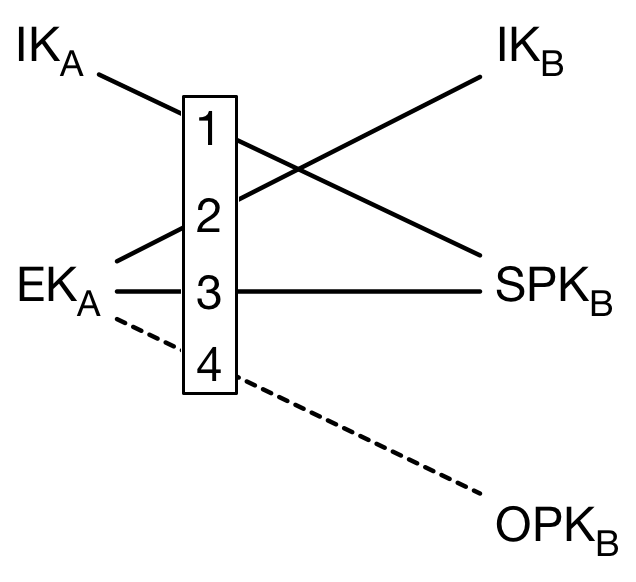
\includegraphics{figures/tripledh.png}
	\caption{Calculations of DH1-DH4 \cite{tripledh}.}
	\label{fig:tripledh}
\end{figure}


\paragraph{Receiving initial message}

Phase three of the X3DH is mostly the same as phase two. Bob retrieves
Alice’s initial message which contains Alice’s identity key and ephemeral
key from the message. Bob will then load his identity private key and the
private key(s) corresponding to the signed prekey and one-time prekey that
Alice used.
Bob repeats the same steps with DH and KDF calculations to derive his
own SK and then deletes the DH values the same as Alice did. Afterwards,
he constructs the AD byte sequence, and in the end, tries to decrypt the
initial ciphertext using the SK and AD. The decryption is the only difference
Bob does to what Alice did on her side. If the decryption fails, Bob will
delete the SK and the protocol aborts and the participants need to restart
the protocol from the start.
If the decryption is successful, he gets the information that Alice had
encrypted, and the protocol is complete for Bob. He deletes any onetime
prekey private key that was used during the protocol, to uphold the
forward secrecy and not get it compromised.

\subsubsection{KDF chain}

KDF Chain is a core concept in the Double Ratchet algorithm.
The job of the KDF chain throughout the Double Ratchet session is to
store each parties KDF key for three chains: a root chain, a sending chain, and
a receiving chain.
The KDF chains are both part of the Diffie-Hellman ratchet step and
the Symmetric-key ratchet step. While the parties exchange messages, they
need to exchange new Diffie-Hellman public keys. The secrets from the DH
output become the inputs to the root chain for the KDF chain, and then the output keys from the root chain become new KDF keys for the sending and
receiving chains. This is the Diffie-Hellman ratchet.
The outputs from the Diffie-Hellman ratchet, the sending and receiving
chains advances for each sending and receiving message, by using the
chains as inputs in the KDF and the output keys are then used to encrypt
and decrypt messages. This is called the symmetric-key ratchet.

\begin{figure}[H]
	\centering
	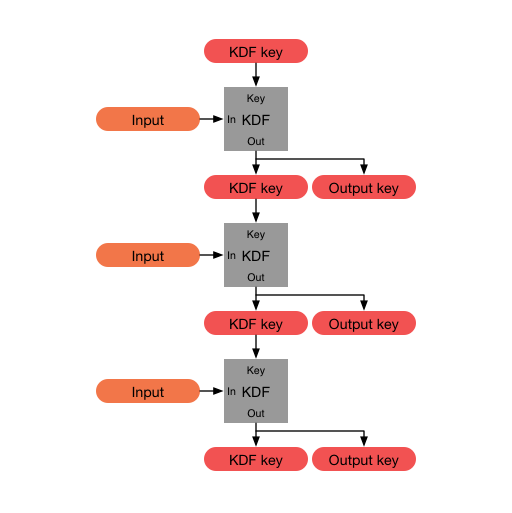
\includegraphics[width=7cm]{figures/kdfchain.png}
	\caption{Processing of three inputs and the resulting outputs in KDF chain \cite{doubleratchet}.}
	\label{fig:kdfchain}
\end{figure}

\subsubsection{Symmetric ratchet}
The symmetric-key ratchet uses KDF chains for its sending and receiving
chains. The output keys are unique message keys which are used to either
encrypt or decrypt messages. The KDF keys for the symmetric-key ratchet
chains will be called chain keys throughout the rest of the Double Ratchet
description.
The KDF chains used for the sending and receiving chains are constant;
they do not need to be random or a secret because the chain key is derived
from the Diffie-Hellman KDF chain which is cryptographically secure. The
documentation explains the constant can be a single byte 0x01 for the
message key and then a single byte 0x02 for the chain key. The sending
and receiving chains ensure that each message is encrypted or decrypted
with a unique key and can be deleted after use. There is only a single
symmetric-key ratchet step to calculate a new message and chain key from
an already given chain key. The diagram below shows two steps in this
process. The first KDF gets a chain key from the Diffie-Hellman KDF chain
and outputs a new chain key for the next KDF and a message key to encrypt
or decrypt a message.

\begin{figure}[H]
	\centering
	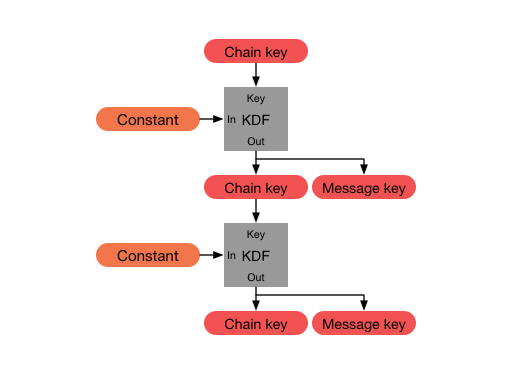
\includegraphics[width=10cm]{figures/symmetrickeyratchet.png}
	\caption{Symmetric key ratchet \cite{doubleratchet}.}
	\label{fig:symkeyratchet}
\end{figure}

The message key that is derived from the KDF chain is not used later on to derive new message keys or chaining keys. Because of this, it is fully
possible to store the message key without affecting the security of other
keys, only the message that belongs to the particular message key. It is
quite useful when the protocols handles out-of-order messages because a
participant can store the message key and decrypt the message later when
they receive the correct message for that message key.

\subsubsection{Deffie-Hellman ratchet}
The Double Ratchet is formed by combining the symmetric-key ratchet and
the Diffie-Hellman ratchet. If the Double Ratchet did not use the Diffie-
Hellman ratchet to compute new chain keys for the sending and receiving
chain keys, an attacker could steal one of the chain keys and then compute
all future message keys and decrypt all future messages.
For this to work, each party generates a DH key pair, a public and a
private key, which will be their first ratchet key pair. When a message
is sent, the header must contain the current public key. When a message
is received, the receiver checks the public keys that are given with the
message and do a DH ratchet step to replace the receiver’s current ratchet
key pair with a new one.
The result is a kind of ”ping-pong” behavior as the two parties take
turns replacing their key pairs. The attacker will have a harder time to get
any valuable information from the parties, since if one of the messages gets
compromised, and the attacker learns the value of the current private key,
it will not make any difference since the private key will soon be replaced
with a new, uncompromised key.
From this point onwards, this section will present an example of how
the Diffie-Hellman ratchet works to get a shared sequence of DH outputs.
The initialization starts with Bob sending his ratchet public key to Alice,
while Bob does not know Alice’s ratchet public key. Alice will now do
the initialization step by performing a DH calculation between her ratchet
public key and Bobs ratchet public key.
Figure

\begin{figure}[H]
	\centering
	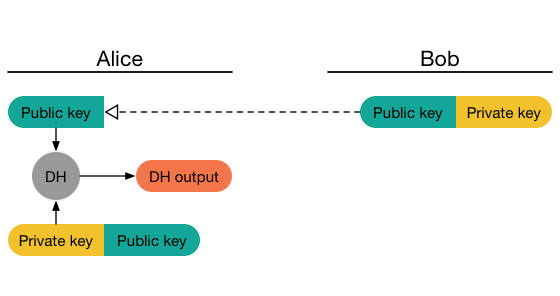
\includegraphics[width=10cm]{figures/dhratchet1.png}
	\caption{Diffie-Hellman ratchet 1 \cite{doubleratchet}.}
	\label{fig:dhratchet1}
\end{figure}

The figure shows Alice advertise her ratchet public key to Bob after she
is done with her Diffie-Hellman calculation. When Bob receives Alice’s
initial message, he performs a Diffie-Hellman ratchet step by calculating
the new DH output between Alice’s ratchet public key and his ratchet private key, which equals Alice’s DH output. The DH outputs are equal
because the figures are a simplification of the DH ratchet, and there is a
KDF chain which uses a Root Key (shared secret between Alice and Bob) to
output the same keys. He then replaces his ratchet key pair and calculates
a new DH output.

\begin{figure}[H]
	\centering
	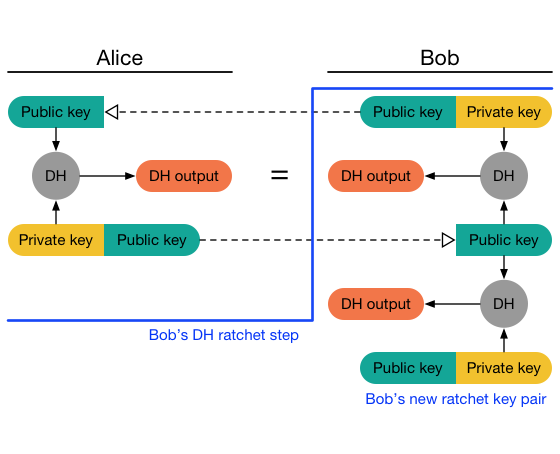
\includegraphics[width=10cm]{figures/dhratchet2.png}
	\caption{Diffie-Hellman ratchet 2 \cite{doubleratchet}.}
	\label{fig:dhratchet2}
\end{figure}

Bob sends his next message with the new ratchet public key. Eventually,
Alice receives Bob’s new message with his new ratchet public key. Alice
derives a newDHoutput with her ratchet private key and Bob’s new public
key to get the same DH output as Bob for decrypting the message and then
generates a new DH ratchet key pair to replace her old key pair. With the
new DH ratchet key pair, Alice derives another DH output with her new
ratchet private key and the same ratchet public key from Bob, which is used
in the next message exchange. These exchanges continue for each message
sent with a new ratchet public key and new DH output.

%\begin{figure}[H]
%	\centering
%	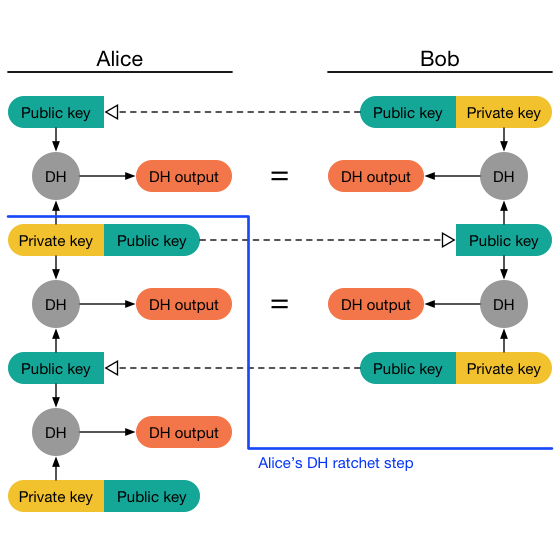
\includegraphics[width=10cm]{figures/dhratchet3.png}
%	\caption{Diffie-Hellman ratchet 3 \cite{doubleratchet}.}
%	\label{fig:dhratchet3}
%\end{figure}

\begin{figure}[H]
	\centering
	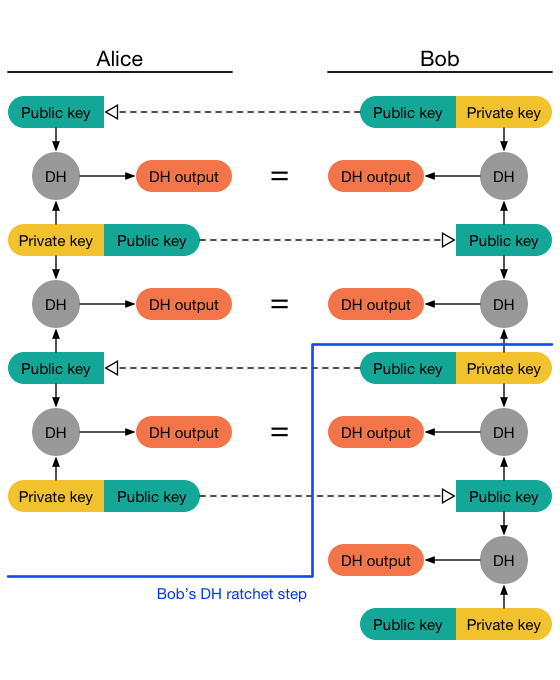
\includegraphics[width=10cm]{figures/dhratchet4.png}
	\caption{Diffie-Hellman ratchet 4 \cite{doubleratchet}.}
	\label{fig:dhratchet4}
\end{figure}

Until now the DH outputs have only been called outputs to simplify the
description of the DH ratchet, but the DH outputs are used in a KDF to get
the sending and receiving chain keys for the symmetric-key ratchet. Figure
3.5 shows the DH outputs are changed with sending or receiving chains.
The first time Alice sends out her message with her ratchet public key and
DH output, a sending chain is derived from the DH output through a KDF
chain, and Bob on his side derives a receiving chain key from hisDHoutput
by using Alice’s public key and his private key. Bob then derives a new
sending chain key from his second DH output.


\begin{figure}[H]
	\centering
	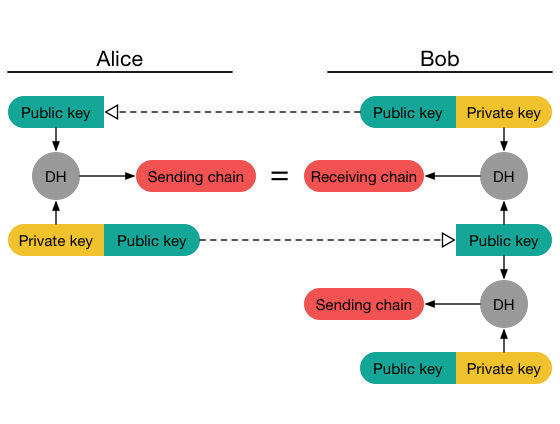
\includegraphics[width=10cm]{figures/dhratchet5.png}
	\caption{Diffie-Hellman ratchet 5 \cite{doubleratchet}.}
	\label{fig:dhratchet5}
\end{figure}



The figures shown until now have been a simplification of the DH
ratchet. The DH ratchet takes the output keys and uses them as KDF inputs
to a root chain, and then the KDF outputs are used as a sending or receiving
key. Using a KDF chain here improves the resilience and break-in recovery.
Figure 3.6 shows that the DH ratchet updates the root KDF chain twice, and
uses the KDF output keys as new sending and receiving chain keys

%\begin{figure}[H]
%	\centering
%	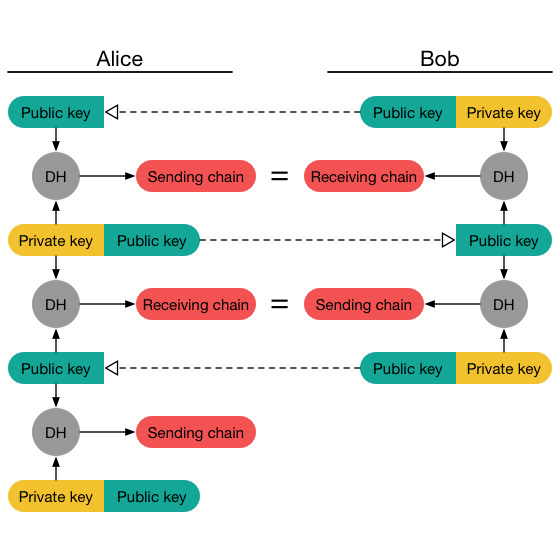
\includegraphics[width=10cm]{figures/dhratchet6.png}
%	\caption{Diffie-Hellman ratchet 6 \cite{doubleratchet}.}
%	\label{fig:dhratchet6}
%\end{figure}

\begin{figure}[H]
	\centering
	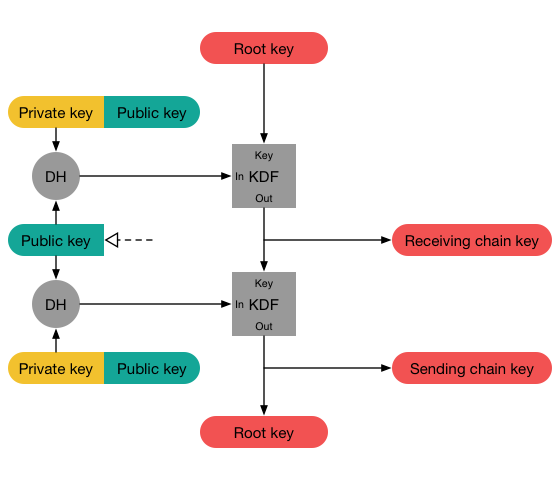
\includegraphics[width=10cm]{figures/dhratchet7.png}
	\caption{Diffie-Hellman ratchet 7 \cite{doubleratchet}.}
	\label{fig:dhratchet7}
\end{figure}

\subsubsection{Double ratchet}
Double Ratchet is the algorithm we get by combining symmetric-key
ratchet and Diffie-Hellman ratchet. 
When a message is sent or received, a symmetric-key ratchet step is
applied to the sending or receiving chain to derive the message key.
When a new ratchet public key is received, a DH ratchet step is performed prior to the symmetric-key ratchet to replace the chain keys.

This section is about how these algorithms work together to form the
Double Ratchet, seen from Alice’s perspective. The figure shows after Alice
has done her initialization with Bob’s ratchet public key, and the Root Key
(RK) is the shared secret used as the initial root key for the KDF chain.
Alice generates her ratchet key pair and then sends the DH output to
the root KDF chain to calculate a new root key and a sending chain key
(CK). The figure is split up into four different parts. The ratchet is
where the ratchet key pair changes and sends Alice’s ratchet private key
and Bob’s ratchet public key to generate a DH output for the root KDF
chain input. The sending column is where the message key for encryption
generates through the symmetric-key KDF chain. The last column is where
the message key for decrypting the received message gets also derived by
the symmetric-key KDF chain. To ensure that the secrecy throughout the
Double Ratchet is upheld, the old RK gets deleted after it has been used to
derive a new RK.

\begin{figure}[H]
	\centering
	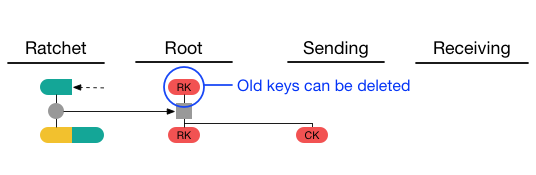
\includegraphics[width=10cm]{figures/doubleratchet1.png}
	\caption{Double ratchet 1 \cite{doubleratchet}.}
	\label{fig:doubleratchet1}
\end{figure}

The next figure shows Alice sending her first message to Bob, message A1.
The sending CK is used on a symmetric-key ratchet step to derive a new
CK and a message key, A1, to encrypt her message. The new CK is stored
for later use, while the old CK and the message key can be deleted since it
no longer is of any use to Alice.

\begin{figure}[H]
	\centering
	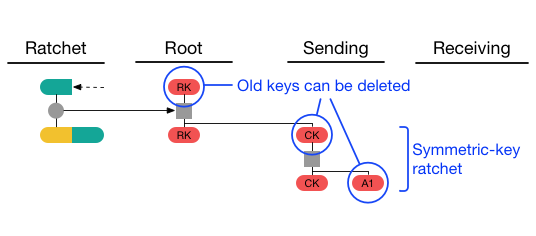
\includegraphics[width=10cm]{figures/doubleratchet2.png}
	\caption{Double ratchet 2 \cite{doubleratchet}.}
	\label{fig:doubleratchet2}
\end{figure}

The figure shows Alice receiving her first response from Bob, message
B1, and he has sent his new ratchet public key, which means Alice needs
to calculate a new ratchet key pair. Alice applies a new DH ratchet step to
derive a new receiving and sending chain keys. Alice uses her old ratchet
private key and Bob’s new public key, to derive a new RK and a CK for
the receiving KDF chain. The receiving chain key is used to derive a new
receiving chain key and a message key to decrypt Bob’s message. Then she
derives a new DH output for the next root KDF chain with her new ratchet
private key to derive a new RK and a sending CK.

\begin{figure}[H]
	\centering
	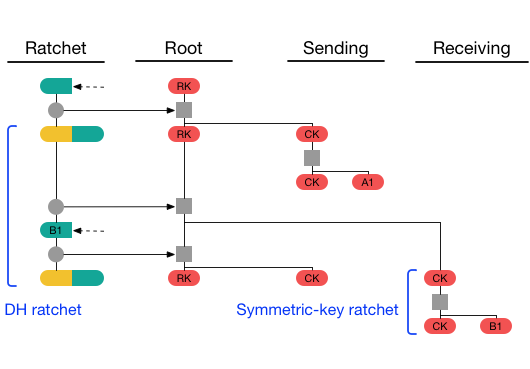
\includegraphics[width=10cm]{figures/doubleratchet3.png}
	\caption{Double ratchet 3 \cite{doubleratchet}.}
	\label{fig:doubleratchet3}
\end{figure}

The next figure shows how many ratchet steps Alice does when
sending a message A2, receiving a message B2 with Bob’s old ratchet public
key, and then send two new messages A3 and A4 to Bob. Alice received
a message B2 with Bob’s old ratchet keys, which means that Alice only
needs to do a symmetric-key ratchet step to derive a new receiving CK
and a message key to decrypt message B2. Before Alice sends her second
message A2, she needs to do a symmetric-key ratchet step to derive a new
sending CK and a message key to encrypt her message A2. The same must
be done with message A3 and A4, by ratcheting the symmetric-key ratchet
two more times to derive the correct message keys.

\begin{figure}[H]
	\centering
	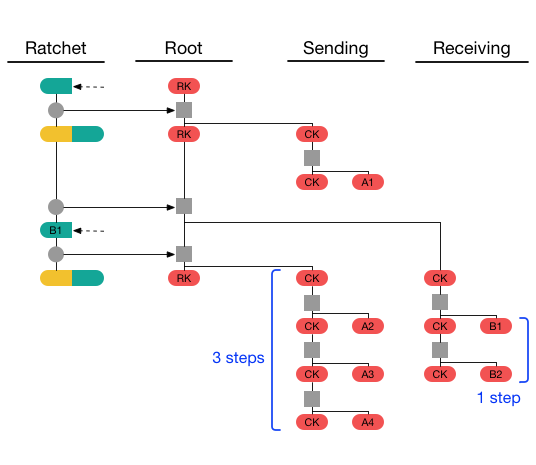
\includegraphics[width=10cm]{figures/doubleratchet4.png}
	\caption{Double ratchet 4 \cite{doubleratchet}.}
	\label{fig:doubleratchet4}
\end{figure}

This figure shows the state when Alice receives messages B3 and B4
from Bob with his new ratchet public key, and the sending of Alice’s last
message, A5. Alice receives new messages from Bob with his new ratchet
public key, and she first derives a new DH output to ratchet the root KDF
chain to get a new RK and a new receiving CK to decrypt Bob’s messages.
The receiving CK is used to run the symmetric-key ratchet step two times,
ones to derive a new CK and a new message key for decryption of message
B3 and then another ratchet step to derive the second CK and message key
for message B4. Alice generates a new ratchet key pair and uses her new
ratchet private key to derive a new RK and a new sending CK with Bob’s
new ratchet public key. The sending CK is used to do a symmetric-key
ratchet step to derive a new CK and a message key to encrypt her new
message, A5.

\begin{figure}[H]
	\centering
	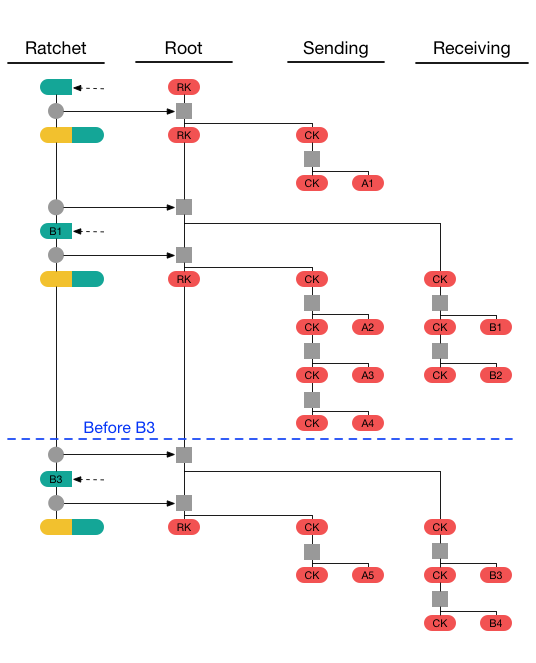
\includegraphics[width=10cm]{figures/doubleratchet5.png}
	\caption{Double ratchet 5 \cite{doubleratchet}.}
	\label{fig:doubleratchet5}
\end{figure}


\subsubsection{Olm}

\subsubsection{Megolm}


\newpage
\section{Information Flow Control} %mere konkret og teknisk
%Selvom jeg ikke kiggr på fx trafic analysis så er det vigtigt at nævne og påpege det ikkeer noget jeg løser

\subsection{The Lattice Model}
adsadsad

\subsection{Noninterference}
dasdsa

\subsection{Static policies}


sadsad
\subsection{Dynamic policies}
sadsadsad


\subsection{Declassification}
Taking some specific information and changing it to a lower security classification.

Identify: What to classify, who declassifies, where the declassification happens and when the declassification happens

\section{Summary}
